There are two parts to the dataset to be collected.

The first is "candidate" time series. The candidates consist of the letters of the alphabet, written in both uppercase and lowercase. Each letter will be replicated five times, for a total of 260 recordings per person. Around 100 people will participate in the instrument for a total of 26000 recordings.

The second part is "data" time series. The data time series are words to be tested. These words will be taken from Lincoln's Gettsyburg Address: "Four score and seven years ago our fathers brought forth on this continent, a new nation, conceived in Liberty, and dedicated to the proposition that all men are created equal." Each word will be recorded individually. This will also be replicated by 100 people, for a total of 30000 recordings.

Thus, the total size of the dataset will be 56000.

The data will be recorded with the LEAP Motion, using a browser application. \\
\begin{figure}
  \begin{center}
  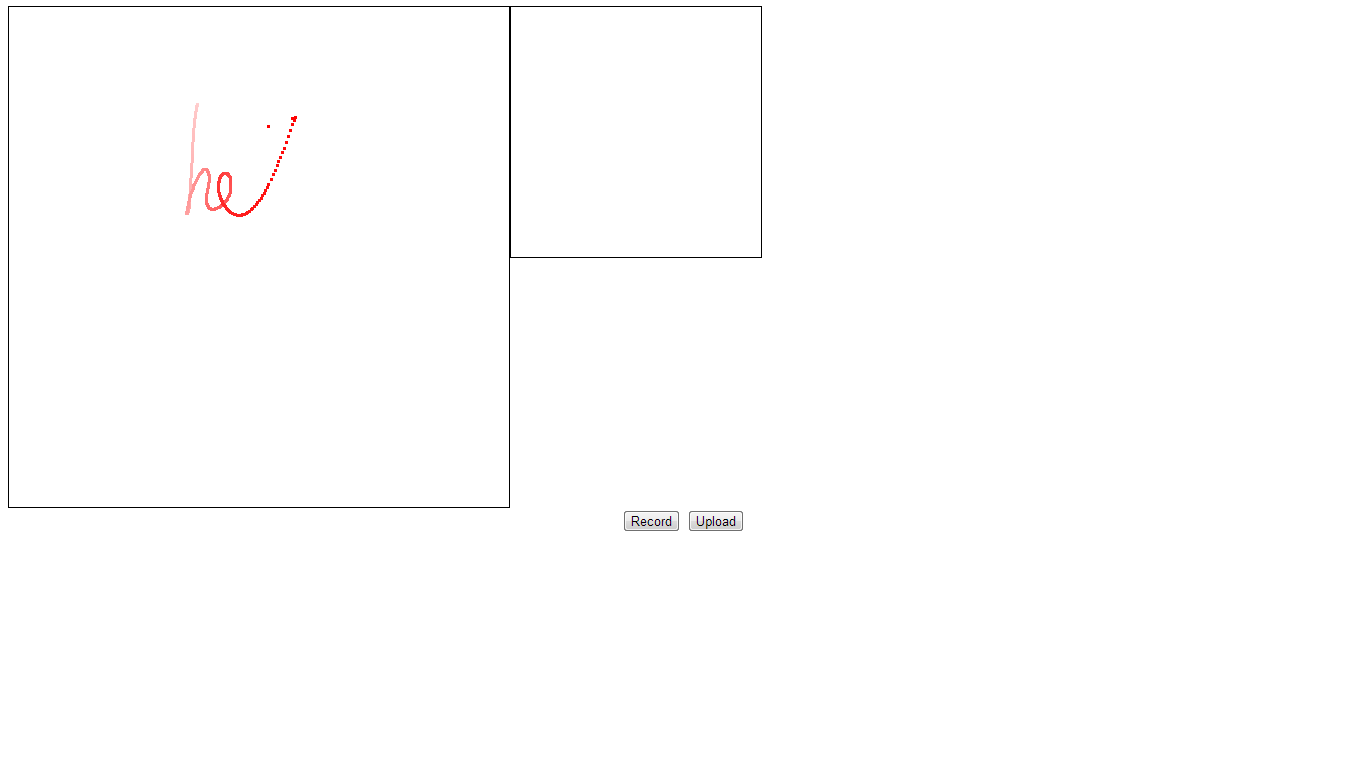
\includegraphics[width=\columnwidth]{images/recording-1.PNG}
  \caption{The data recording apparatus}
  \label{fig:teaser}
  \end{center}  
\end{figure}
The browser application shows a 2D preview of the data being recorded and prompts users to confirm the character or word they just wrote.
After the user has finished recording, the data will be uploaded, so at this stage, the user requires an internet connection.
